\documentclass[10pt]{article}
\usepackage{amsmath,amssymb}
\setlength{\oddsidemargin}{0in}
\setlength{\evensidemargin}{0in}
\setlength{\textheight}{9in}
\setlength{\textwidth}{6.5in}
\setlength{\topmargin}{-0.5in}
\usepackage{enumitem}
\usepackage{graphicx}
\usepackage{float}
\DeclareMathOperator*{\argmax}{arg\,max}
\DeclareMathOperator*{\argmin}{arg\,min}
\title{\bf Math 170S: Homework 1}
\date{10/20/2023}
\author{\bf Owen Jones}

\begin{document}
\maketitle
\begin{enumerate}[label=\textbf{Problem \arabic*.}]
    \item $f(x)=\frac{\lambda^x}{x!}e^{-\lambda}$
        $P(X_1=x_1,X_2=x_2,\ldots,X_n=x_n)=P(X_1=x_1)P(X_2=x_2)\ldots P(X_n=x_n)$ by independence. Thus, $L(x_1,x_2,\ldots,x_n,\lambda)=\displaystyle\prod_{i=1}^{n}\frac{\lambda^{x_i}}{x_i!}e^{-\lambda}$.\\
        $\log$ preserves maximization, so $\displaystyle \argmax_\lambda L(x_1,x_2,\ldots,x_n,\lambda)=\argmax_\lambda \log (L(x_1,x_2,\ldots,x_n,\lambda))$.\\
        $\displaystyle \argmax_\lambda L(x_1,x_2,\ldots,x_n,\lambda)=\sum_{i=1}^{n}\log(\frac{\lambda^{x_i}}{x_i!}e^{-\lambda})=\sum_{i=1}^{n}x_i\log(\lambda)-\log(x_i!)-\lambda$
        $\frac{\partial L}{\partial \lambda}=0=\displaystyle \sum_{i=1}^{n}\frac{x_i}{\lambda}-1\Rightarrow \hat{\lambda}=\frac{\displaystyle\sum_{i=1}^{n}x_i}{n}=\overline{x}$\\
    We know $L(\hat{\lambda})$ is a maximum by the second derivative test $\displaystyle\frac{\partial^2L}{\partial\lambda^2}=\sum_{i=1}^{n}-\frac{x_i}{\lambda^2}<0$ because the $x_is$ are positive and any number squared is positive.
    \item For $5$ heads and $25$ tails $L(X_1=x_1,X_2=x_2,\ldots X_{30}=x_{30},p)=\displaystyle\prod_{i=1}^{30}p^{x_i}{(1-p)}^{1-x_i}$ for $x_i\in\{0,1\}$.
    $\displaystyle\argmax_p L(p)=\sum_{i=1}^{30}x_i\log(p)+(1-x_i)\log(1-p)$
    $\displaystyle\frac{\partial L}{\partial p}=0=\sum_{i=1}^{30}\frac{x_i}{p}-\frac{1-x_i}{1-p}=\frac{5}{p}-\frac{25}{1-p}\Rightarrow 5(1-p)=25p\Rightarrow \hat{p}=\frac{1}{6}\\$
    We know $L(\hat{\lambda})$ is a maximum by the second derivative test $\displaystyle\frac{\partial^2L}{\partial p^2}=-\frac{5}{p^2}-\frac{25}{{(1-p)}^2}=-216<0$
    \item \begin{itemize}
        \item [1.] WTS $f(x|y,\theta)\ge0$ for all $x$ and $\int_{y}^{\infty}f(x|y,\theta)dx=1$ (using $x\ge y$.)\\
        $f(x|y,\theta)=\theta y^\theta x^{-\theta-1}$. 
        $\theta$ and $y$ are both positive, so $\theta y^\theta>0$. $x\ge y>0$, so $x>0$. 
        A positive number raised to any power is positive, so $x^{-\theta-1}>0$. 
        Hence, $\theta y^\theta x^{-\theta-1}$ for all $x$.\\
        $\displaystyle\int_{y}^{\infty}\theta y^\theta x^{-\theta-1}dx=-y^\theta x^{-\theta}|^\infty_y=-y\lim_{x\rightarrow\infty}x^{-\theta}-(-y^{\theta-\theta})=1$ ($\theta>1$)
        \item [2.] $\displaystyle L(\theta)=\prod_{i=1}^{n}\theta y^\theta x_i^{-\theta-1}$ $\displaystyle \argmax_\theta L(\theta)=\argmax_\theta \log(L(\theta))=\sum_{i=1}^{n}\log(\theta)+\theta\log(y)-(\theta+1)\log(x_i)$.
        $\displaystyle\frac{\partial L}{\partial \theta}=0=\sum_{i=1}^{n}\frac{1}{\theta}+\log(y)-\log(x_i)\Rightarrow\frac{n}{\theta}=\sum_{i=1}^{n}\log(\frac{x_i}{y})\Rightarrow\hat{\theta}=\frac{n}{\displaystyle\sum_{i=1}^{n}\log(\frac{x_i}{y})}$\\
        We know $L(\hat{\theta})$ is a maximum by the second derivative test $\displaystyle\frac{\partial^2L}{\partial\theta^2}=-\frac{n}{\theta^2}<0$ because the square of any number is positive and a negative times a positive is negative.
    \end{itemize}
    \newpage
    \item \begin{itemize}
        \item [1.] $\beta_1=\frac{cov(x,y)}{s_x^2}=\frac{\displaystyle\sum (y-\overline{y})(x-\overline{x})}{\displaystyle\sum {(x-\overline{x})}^2}=1.09878929$, $\beta_0=\overline{y}-b\overline{x}=2.9788896$
        
        \item [2.] \begin{figure}[h!]
            \centering
            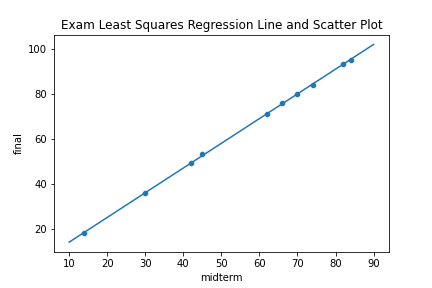
\includegraphics[scale=0.5]{Exam Least Squares Regression Line and Scatter Plot.png}
        \end{figure}
        \item [3.] \begin{figure}[h!]
            \centering
            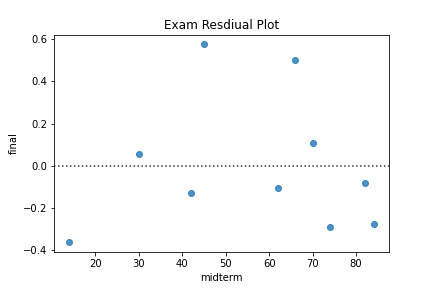
\includegraphics[scale=0.5]{Exam Resdiual Plot.png}
        \end{figure}
        The residuals from the Midterm vs. Final plot don't follow a trend (points are randomly distributed above and below the regression line). This implies a linear regression fits the data well.
        \item [4.] $\displaystyle L(\beta_0,\beta_1,\sigma^2)=\prod_{i=1}^{n}\frac{1}{\sqrt{2\pi\sigma^2}}\exp(-\frac{{(y_i-(\beta_0+\beta_1x_i))}^2}{2\sigma^2})$.
        $\displaystyle\argmax_{\sigma^2}L(\sigma^2)=\log(\argmax_{\sigma^2}L(\sigma^2))=\sum_{i=1}^{n}-\frac{1}{2}\log(2\pi)-\frac{1}{2}\log(\sigma^2)-\frac{{(y_i-(\beta_0+\beta_1x_i))}^2}{2\sigma^2}$
        $\displaystyle\frac{\partial L}{\partial \sigma^2}=0=\sum_{i=1}^{n}-\frac{1}{2\sigma^2}+\frac{{(y_i-(\beta_0+\beta_1x_i))}^2}{2{(\sigma^2)}^2}\Rightarrow\hat{\sigma^2}=\frac{\displaystyle\sum_{i=1}^{n}{(y_i-(\beta_0+\beta_1x_i))}^2}{n}$\\
        We know $L(\hat{\sigma^2})$ is a maximum by the second derivative test $\displaystyle\frac{\partial^2L}{\partial {(\sigma^2)}^2}=\frac{n}{2{(\sigma^2)}^2}-\frac{\sum_{i=1}^{n}{(y_i-(\beta_0+\beta_1x_i))}^2}{{(\sigma^2)}^3}=\frac{n}{2{(\sum_{i=1}^{n}{(y_i-(\beta_0+\beta_1x_i))}^2)}^2}-\frac{n^3}{{(\sum_{i=1}^{n}{(y_i-(\beta_0+\beta_1x_i))}^2)}^2}<0$ because $n^3>\frac{n}{2}$ for all natural numbers and variance is positive.
    \end{itemize}
    \item We need two equations because we have two unknowns.
    $$E[X]=\int_{0}^{1}xf(x|\alpha,\beta)dx=\frac{\alpha}{\alpha+\beta}\int_{0}^{1}\frac{\Gamma(\alpha+\beta+1)}{\Gamma(\alpha+1)\Gamma(\beta)}x^\alpha{(1-x)}^{\beta-1}dx=\frac{\alpha}{\alpha+\beta}\int_{0}^{1}beta(\alpha+1,\beta)dx=\frac{\alpha}{\alpha+\beta}$$
    $$E[X^2]=\int_{0}^{1}x^2f(x|\alpha,\beta)dx=\frac{\alpha(\alpha+1)}{(\alpha+\beta)(\alpha+\beta+1)}\int_{0}^{1}beta(\alpha+2,\beta)dx=\frac{\alpha(\alpha+1)}{(\alpha+\beta)(\alpha+\beta+1)}$$
    $\beta=\frac{{(1-E[X])}^2}{E[X](E[X^2]-E[X]^2)}$
    $\alpha=E[X^2]\frac{1-E[X]}{E[X^2]-E[X]^2}$
\end{enumerate}
\end{document}